
\documentclass[fleqn,addpoints]{exam}

\usepackage{graphicx}
\usepackage{booktabs}
\usepackage{float}
\usepackage{amsmath}
\usepackage{cancel}
\usepackage{polynom}
\usepackage{caption}
\usepackage{mdwlist}

\newcommand{\degree}{\ensuremath{^\circ}} 

% \usepackage{2in1, lscape} 

\title{Math 115 \\ Study Guide}
\date{July 26, 2011} 

\begin{document}

\maketitle

% \begin{figure}[H]
%   \centering
%   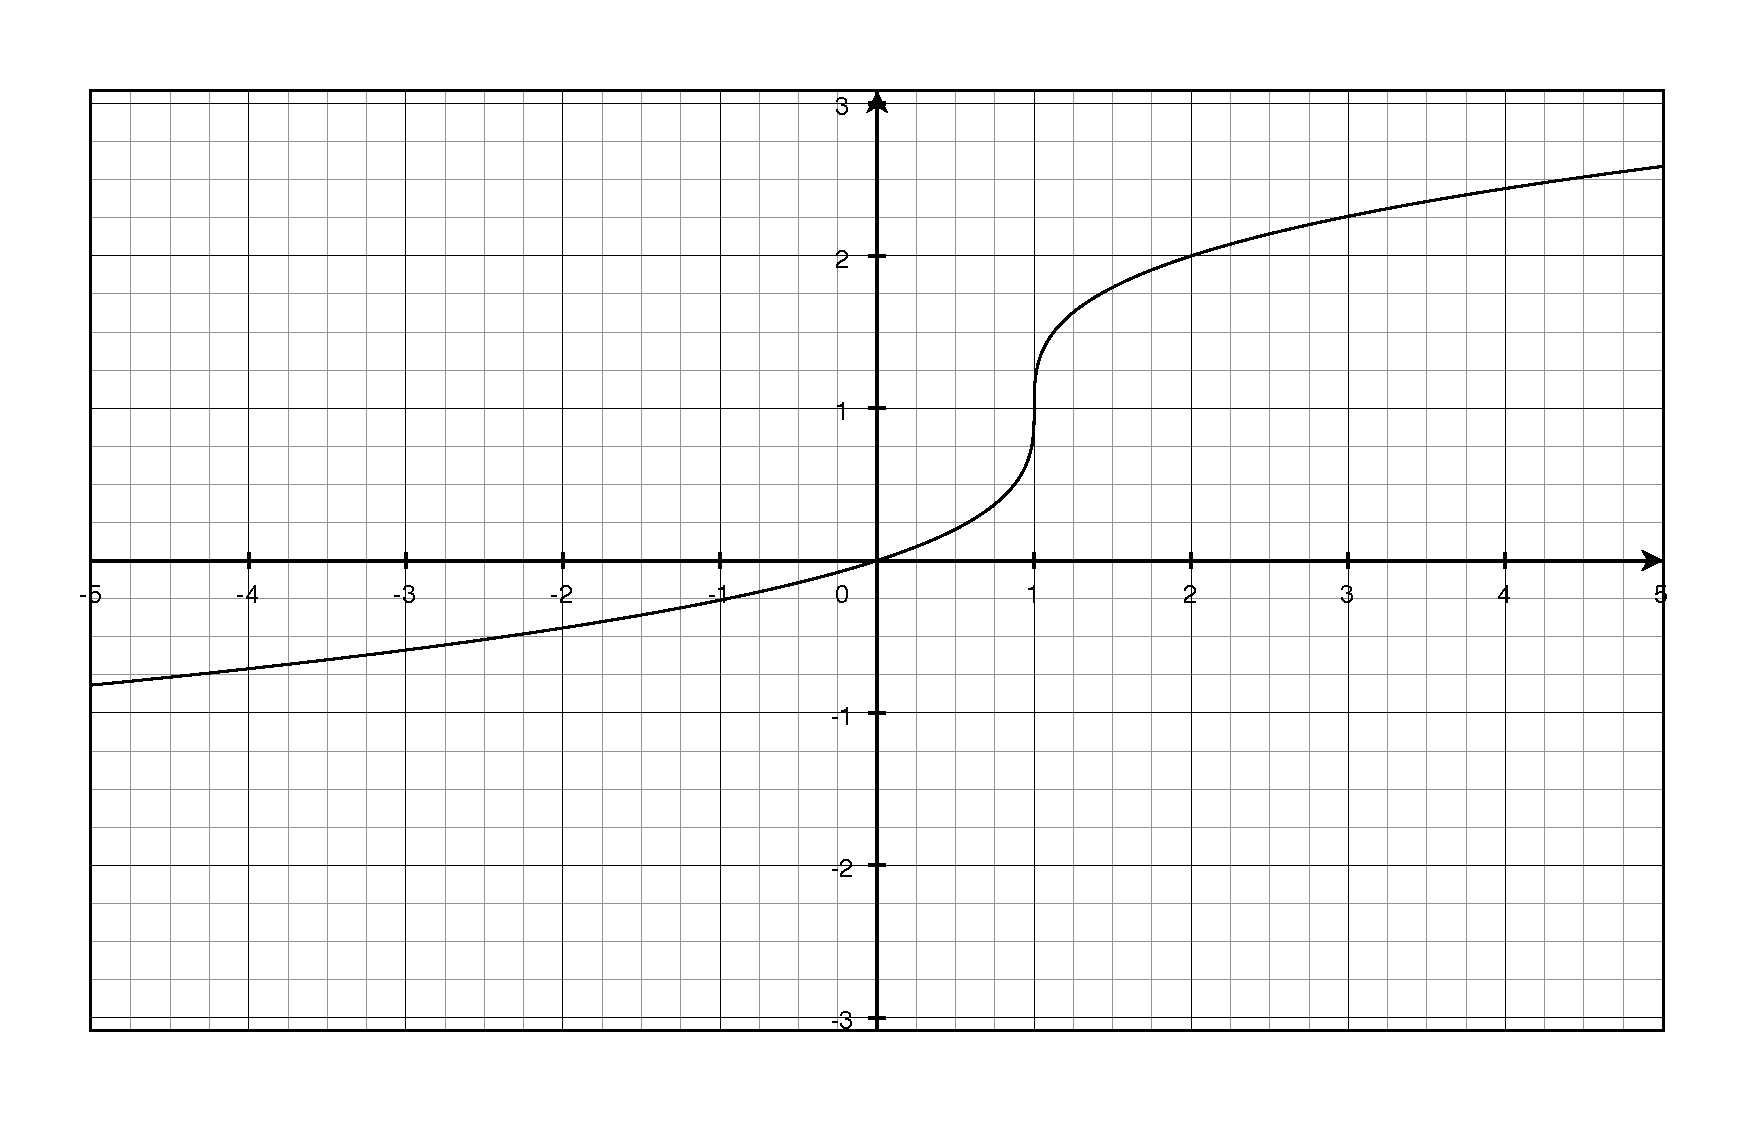
\includegraphics[scale=.3]{question7.eps}
%   \caption*{Question 7}
% \end{figure}

% \begin{tabular}{cc}
% \toprule
% period & amplitude \\
% \midrule
%   $\pi$ & $2$ \\
% \bottomrule
% \end{tabular}

\section{Miscellaneous}

\begin{itemize}
\item Check your work:
  \begin{itemize*}
    \item Plug the answer in the original equation.  
    \item Do the problem again. 
    \item Try to find a second way to solve the same problem.  
  \end{itemize*}
\item There isn't any bonus for finishing early, so use all the time.
\item No matter how complicated an equation looks, the strategy for solving it is usually to factor and then set each
  factor equal to zero.  This strategy applies, when the equation contains $x^2$, $e^{2x}$, $\cos^2 x$, or some
  combination of these.
\end{itemize}

This study guide contains the things I thought of that seemed important.  Of course, I haven't seen the test, so I may have
missed or forgotten something.  The problems are taken from the sample OU exams.

The problems are from the sample midterm and final.  I didn't re-type the problems here, so you need copies of the tests
to know what the problems are.  

\section{Linear Equalities and Inequalities}

\subsection{Things You Should Know}
\begin{itemize}
\item problems with absolute values are actually two problems.  One problem with a negative number inside the absolute
  value sign and one problem with a positive number inside the absolute value sign.
\item some of the solutions you come up with for a problem containing an inequality may not actually work in the original
  equation.  You need to check your solutions and only include the ones that actually work.
\item know how to find the equation a line given two points
\item the slope of a perpendicular line is the negative reciprocal of the original slope
\item ``linear depreciation'' means you need to find a linear equation where the y-axis is money and the x-axis is time.
\end{itemize}

\subsection{Sample Problems}

\begin{description}
\item[Midterm 1]

\begin{align*}
  (2x+1)^2(x+2) \geq 0
\end{align*}

$(2x+1)^2$ is always positive, so the answer is $x \geq -2$

\item[Midterm 2]
\begin{align*}
  (3x+1)(2x+3)(2-x) \geq 0
\end{align*}

The x-intercepts are: $x = -\dfrac{1}{3}$, $x = -\dfrac{2}{3}$, and $x=2$.  If you plug in other values of $x$ around
these points, you find that:
\[
  \left(-\infty, -\frac{3}{2} \right] \cup \left[- \frac{1}{3}, 2 \right ]
\]

\item[Midterm 3]
\begin{align*}
  |2x+3| \geq 2 \\
  \\
  2x+3 \geq 2 & \text{ or } -(2x+3) \geq 2 \\
  2x \geq -1 & \text{ or } 2x+3 \leq -2 \\
  x \geq -\frac{1}{2} & \text{ or } 2x \leq -5 \\
  x \geq -\frac{1}{2} & \text{ or } x \leq -\frac{5}{2} \\
\end{align*}

\[
  \left( -\infty, -\frac{5}{2} \right] \cup \left[-\frac{1}{2}, \infty \right)
\]

\item[Sample Final 2]

\begin{description}

\item[a]
This problem is about finding the equation of a line given two points on the line.  The two points are:

\begin{itemize}
  \item time zero: $(0, 10,000)$.  This is also the y-intercept.
  \item time 6: $(6, 100)$
\end{itemize}

First find the slope:
\[
  m = \frac{10,000 - 100}{0-6} = -1650
\]

Now we know the slope and the y-intercept, so the equation of the line is:
\[
  f(t) = -1650t + 10,000
\]

\item[b]
\[
  f(3) = 5,050
\]

\end{description}

\item[Sample Final 3]

\begin{align*}
  |-2x+5| - 3x &= 2 \\
  |-2x+5| &= 3x + 2 \\
\end{align*}

\begin{align*}
  -2x+5 &= 3x + 2 \\
   x &= \frac{3}{5}
\end{align*}

$\dfrac{3}{5}$ works in the original equation, so this is a solution.

\begin{align*}
  -(-2x+5) &= 3x + 2 \\
   x &= -7
\end{align*}

$-7$ doesn't work in the original equation, so this is not a solution.

\end{description}
 
\section{Complex Numbers}
\subsection{Things You Should Know}
\begin{itemize*}
\item how to add, subtract, multiply, and divide complex numbers
\item how use the {\em complex conjugate}  to simplify a fraction containing complex numbers
\end{itemize*}

\begin{description}
\item[Midterm 14]
\begin{align*}
  (1-3i)(-4-i) = -4 + 12i -i + 3i^2 = -7 + 11i
\end{align*}

\item[Midterm 15]
\begin{align*}
  \frac{1+i}{2-3i} \cdot \frac{2+3i}{2+3i} = \frac{-2}{13} + \frac{5}{13} i
\end{align*}

\end{description}

\section{Functions}

\subsection{Things You Should Know}
\begin{itemize*}
\item how to find the domain
\item how to find the range
\item how to find $(f \circ g)(x)$ and the difference between this and $f(x) \cdot g(x)$
\item what happens to the graphs for:
\begin{itemize}
  \item $f(x \pm c)$ (shift left and right)
  \item $f(x) \pm c$ (shift up and down)
  \item $f(c \cdot x) \pm c$ (x-axis scale)
  \item $c \cdot f(x) \pm c$ (y-axis scale)
\end{itemize}

\end{itemize*}

\subsection{Sample Problems}
\begin{description}

\item[Sample Final 4]

To find the inverse:
\begin{itemize*}
  \item solve for $y$
  \item swap $x$ and $y$
\end{itemize*}

\begin{align*}
  y &= \frac{3x-5}{2x+1} \\
  2xy + y &= 3x - 5 \\
  2xy - 3x &= -y - 5 \\
  x &= \frac{-y-5}{2y-3} \\
\end{align*}

So $f^{-1}(x) = \dfrac{-x-5}{2x-3}$

\end{description}

\section{Polynomials}

\subsection{Things You Should Know}
\begin{itemize*}
\item How to use {\em complete the square} to put a quadratic equation in standard form so you can get the vertex from the equation.
\item The minimum or maximum of a parabola is at the vertex, so you find the minimum or maximum by putting the equation
  in standard form.
\item the quadratic formula
\item polynomial long division
\item synthetic long division
\item how to construct a polynomial, given the zeros and a point
\item the {\em Rational Zero Test}
\item complex zeros occur in conjugate pairs
\item Descarte's {\em Rule of Signs}
\item The degree of a polynomial is the largest exponent.
\item Graphs of polynomials with even degree look basically like graphs of $y= \pm x^2$.
\item Graphs of polynomials with odd degree look basically like graphs of $y= \pm x^3$.
\item All the terms after the term with the highest degree determine shape of the graph around the origin, but don't
  affect the graph much for very large or very small values of $x$.
\end{itemize*}

\subsection{Sample Problems}
\begin{description}

\item[Midterm 10]
\begin{align*}
  P(x) &= a(x+1)(x-2)(x-1)^2(x+2)^2 \\
  8 &= a(1)(-2)(-1)^2(2)^2 \\
  a &= -1 \\
  \\
  P(x) &= -(x+1)(x-2)(x-1)^2(x+2)^2 \\
\end{align*}

\item[Sample Final 1]
To find the maximum, you need to complete the square to put the equation in standard form and find the vertex.  I left
out the actual complete the square steps in the typed solutions, but I did them on paper.

\begin{description}
\item[a]
\begin{align*}
  y &= -3x^2 - 7x + 1 \\
  y - \frac{61}{12}   &= -3 \left( x+\frac{7}{6} \right)^2
\end{align*}

So the maximum occurs at the point $\left( -\dfrac{7}{6}, \dfrac{61}{12} \right)$.  

I think this problem may have a typo, since it is much harder than part b.

\item[b]
\begin{align*}
  y &= x^2 + 8x + 5 \\
  y + 11 &= (x+4)^2 \\
\end{align*}

The maximum occurs at: $(-4, -11)$.

\end{description}

\item[Midterm 16]
\[
  x^3 - 3x + 2 = 0
\]

Using the {\em Rational Zero Test} and {\em synthetic long division}, we can identify $(x+2)$ as one factor.

This leaves us with:
\begin{align*}
  (x+2)(x^2 - 2x + 1) &= 0 \\
  (x+2)(x-1)^2 &= 0 \\
\end{align*}

\[
  x = \{-2, 1\}
\]

check:
\begin{align*}
  (-2)^3 - 3(-2) + 2 = -8 + 6 + 2 = 0 \\
  1^3 - 3(1) + 2 = 1 -3 + 2 = 0 \\
\end{align*}

\end{description}


\section{Rational Functions}
\subsection{Things You Should Know}

\begin{itemize*}
\item Find x-intercepts by setting the numerator to zero and solving for x.
\item Find y-intercept by evaluating $f(0)$
\item Find vertical asymptotes by setting the denominator to zero and solving for x.
\item There are two cases for horizontal asymptotes
\begin{itemize}
  \item if the degree of the denominator is greater than the degree of the numerator, there is a horizontal asymptote at
    $y=0$.  This happens because as $x$ gets large, the denominator gets large much more quickly than the numerator.

  \item if the degree of the denominator is the same as the degree of the numerator, there is a horizontal asymptote
    which is obtained using the coefficients from the largest degree term in the numerator and denominator and
    denominator polynomials.  This happens because as $x$ gets large, all the terms other than the terms with the
    largest degree don't matter much.
\end{itemize}

\item There is a slant asymptote if the degree of the numerator is exactly one larger than the degree of the
  denominator.  You find the slant asymptote using long division.

\end{itemize*}

\subsection{Sample Problems}
\begin{description}
\item[Sample Final 5]
\[
  f(x) = \frac{x+3}{2x+1}
\]

\begin{itemize}
  \item x-intercept: $(-3, 0)$
  \item y-intercept: $(0, 3)$
  \item vertical asymptote: $x = -\dfrac{1}{2}$
  \item horizontal asymptote: $y = \dfrac{1}{2}$
\end{itemize}

\begin{figure}[H]
  \centering
  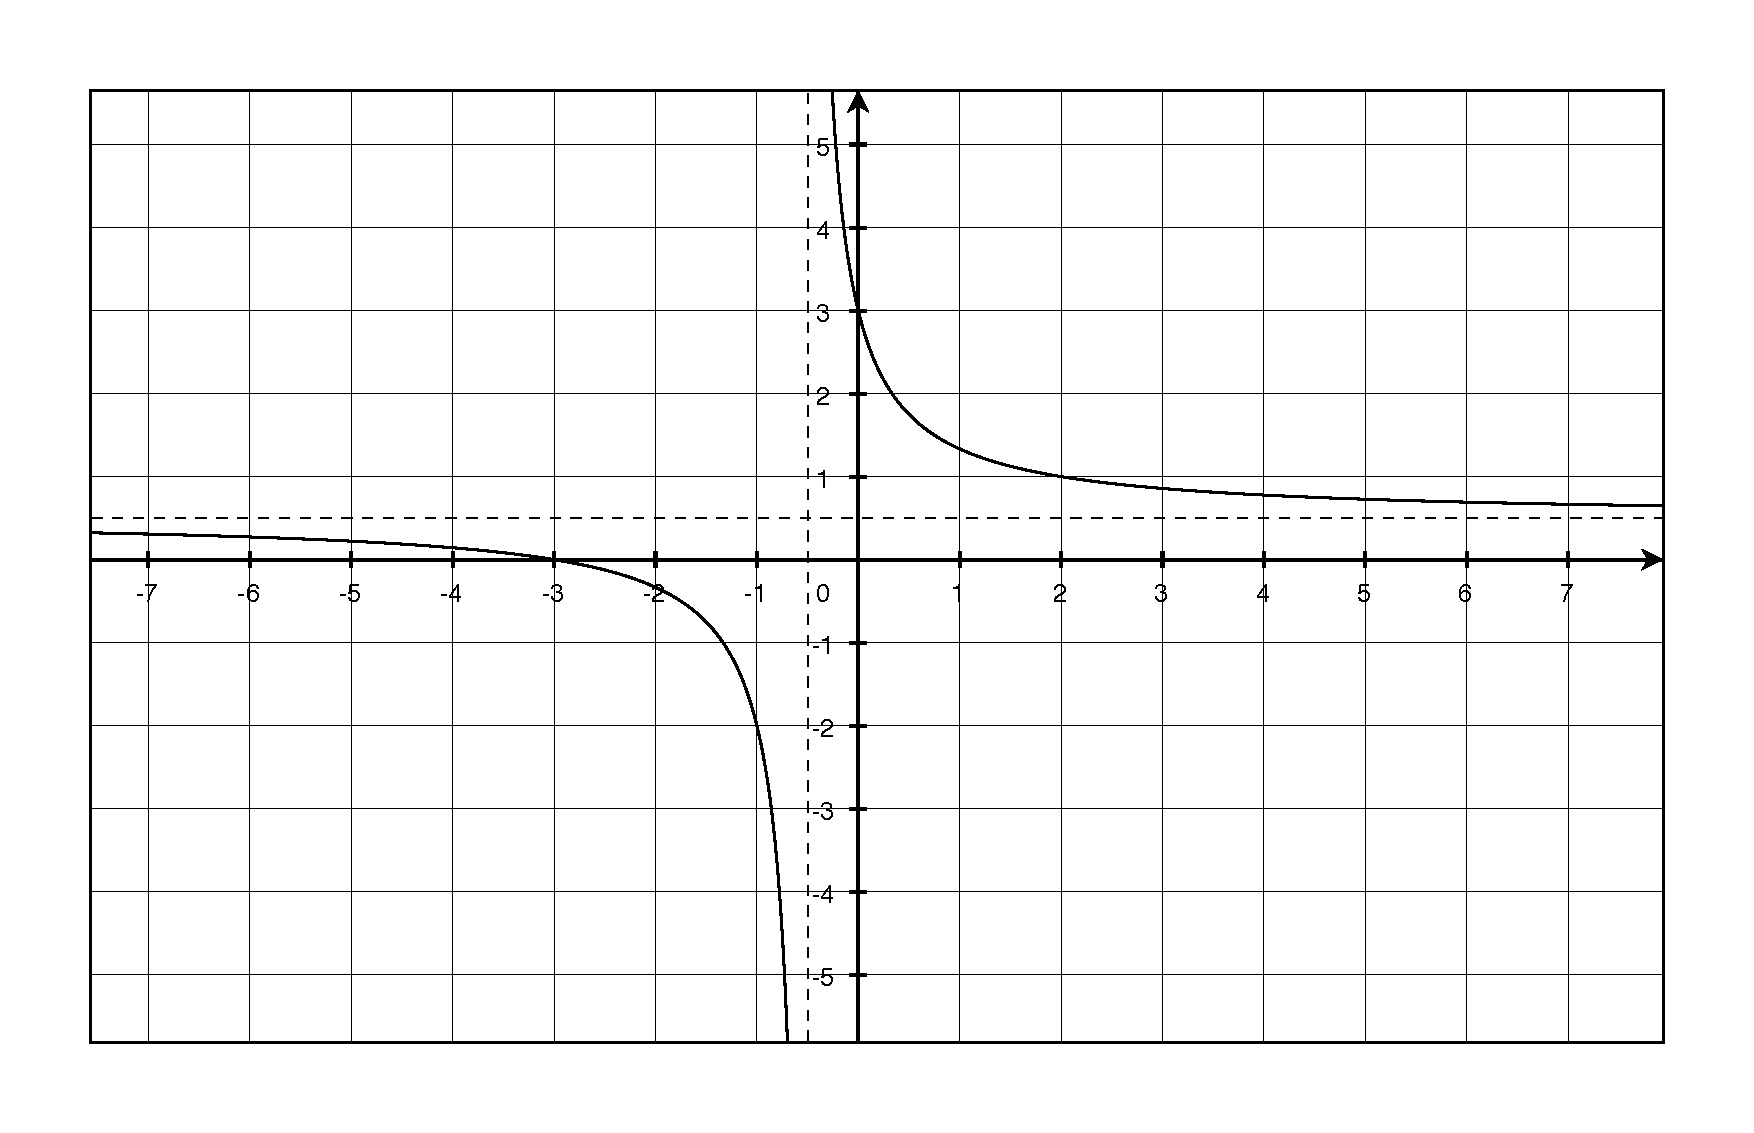
\includegraphics[scale=.5]{final_5.eps}
  \caption*{Final 5}
\end{figure}

\item[Midterm 11]
\[
  f(x) = \frac{(2x-2)(1-x)}{(-2x+1)(x+1)}
\]

\begin{itemize*}
\item x-intercept: $(1, 0)$
\item y-intercept: $(0, -2)$
\item vertical asymptotes: $x = \dfrac{1}{2}$ and $x = -1$
\item horizontal asymptote: $y=1$
\end{itemize*}

The graph is tricky because it doesn't cross the x-axis at the x-intercept.  It just touches and changes direction.  You
can discover this by plugging in an additional point between the x intercept and the vertical asymptote at 
$x = \dfrac{1}{2}$.

\begin{figure}[H]
  \centering
  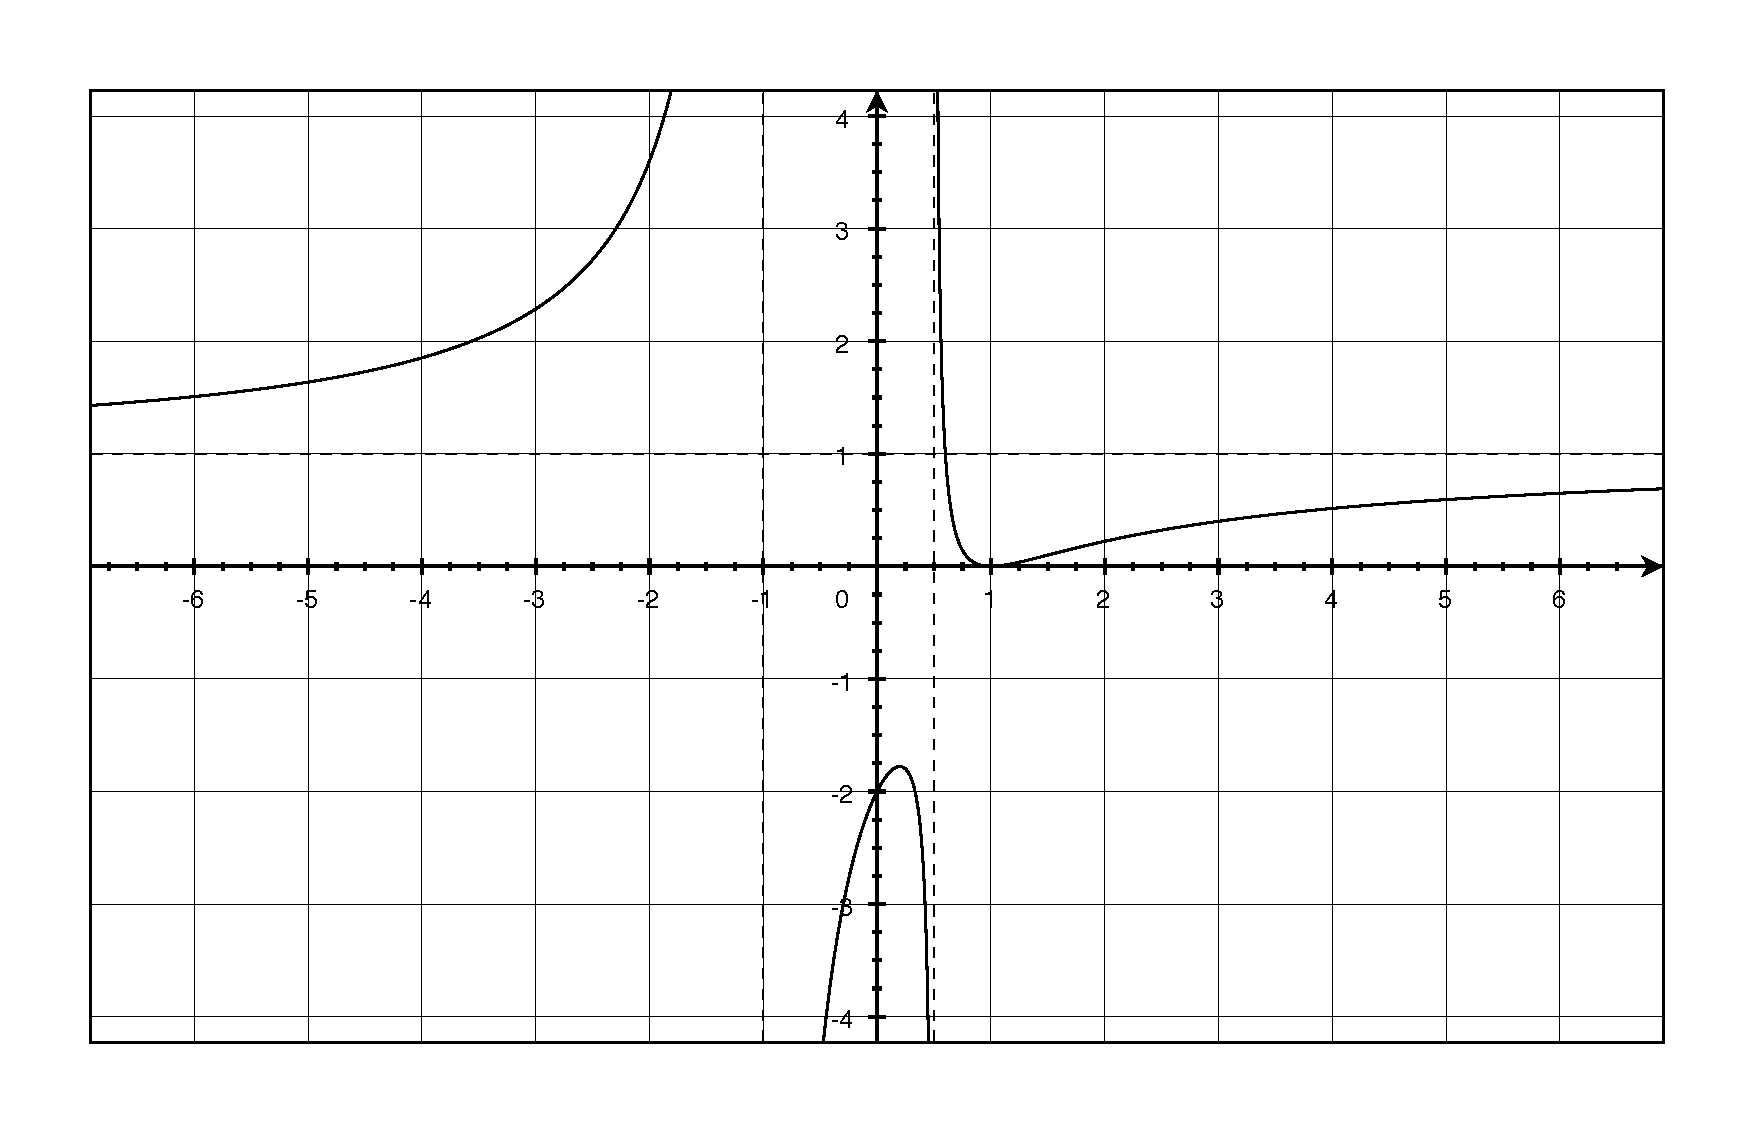
\includegraphics[scale=.5]{midterm_11.eps}
  \caption*{Midterm 11}
\end{figure}

\end{description}

\section{Exponentials and Logarithms}
\subsection{Things You Should Know}
\begin{itemize*}
\item what graphs of $y=c^x$ and $y = \log_c x$ look like
\item rules for simplifying expressions containing logarithms
\item rules for changing bases
\item expression for interest compounded periodically
\item expression for interest compounded continuously
\end{itemize*}

\subsection{Sample Problems}

\begin{description}

\item[Sample Final 6]
\[
 y = 3^{-x} - 1
\]

\begin{itemize*}
  \item domain: $(-\infty, \infty)$
  \item range: $(-1, \infty)$
  \item horizontal asymptote: $y = -1$
\end{itemize*}

\begin{figure}[H]
  \centering
  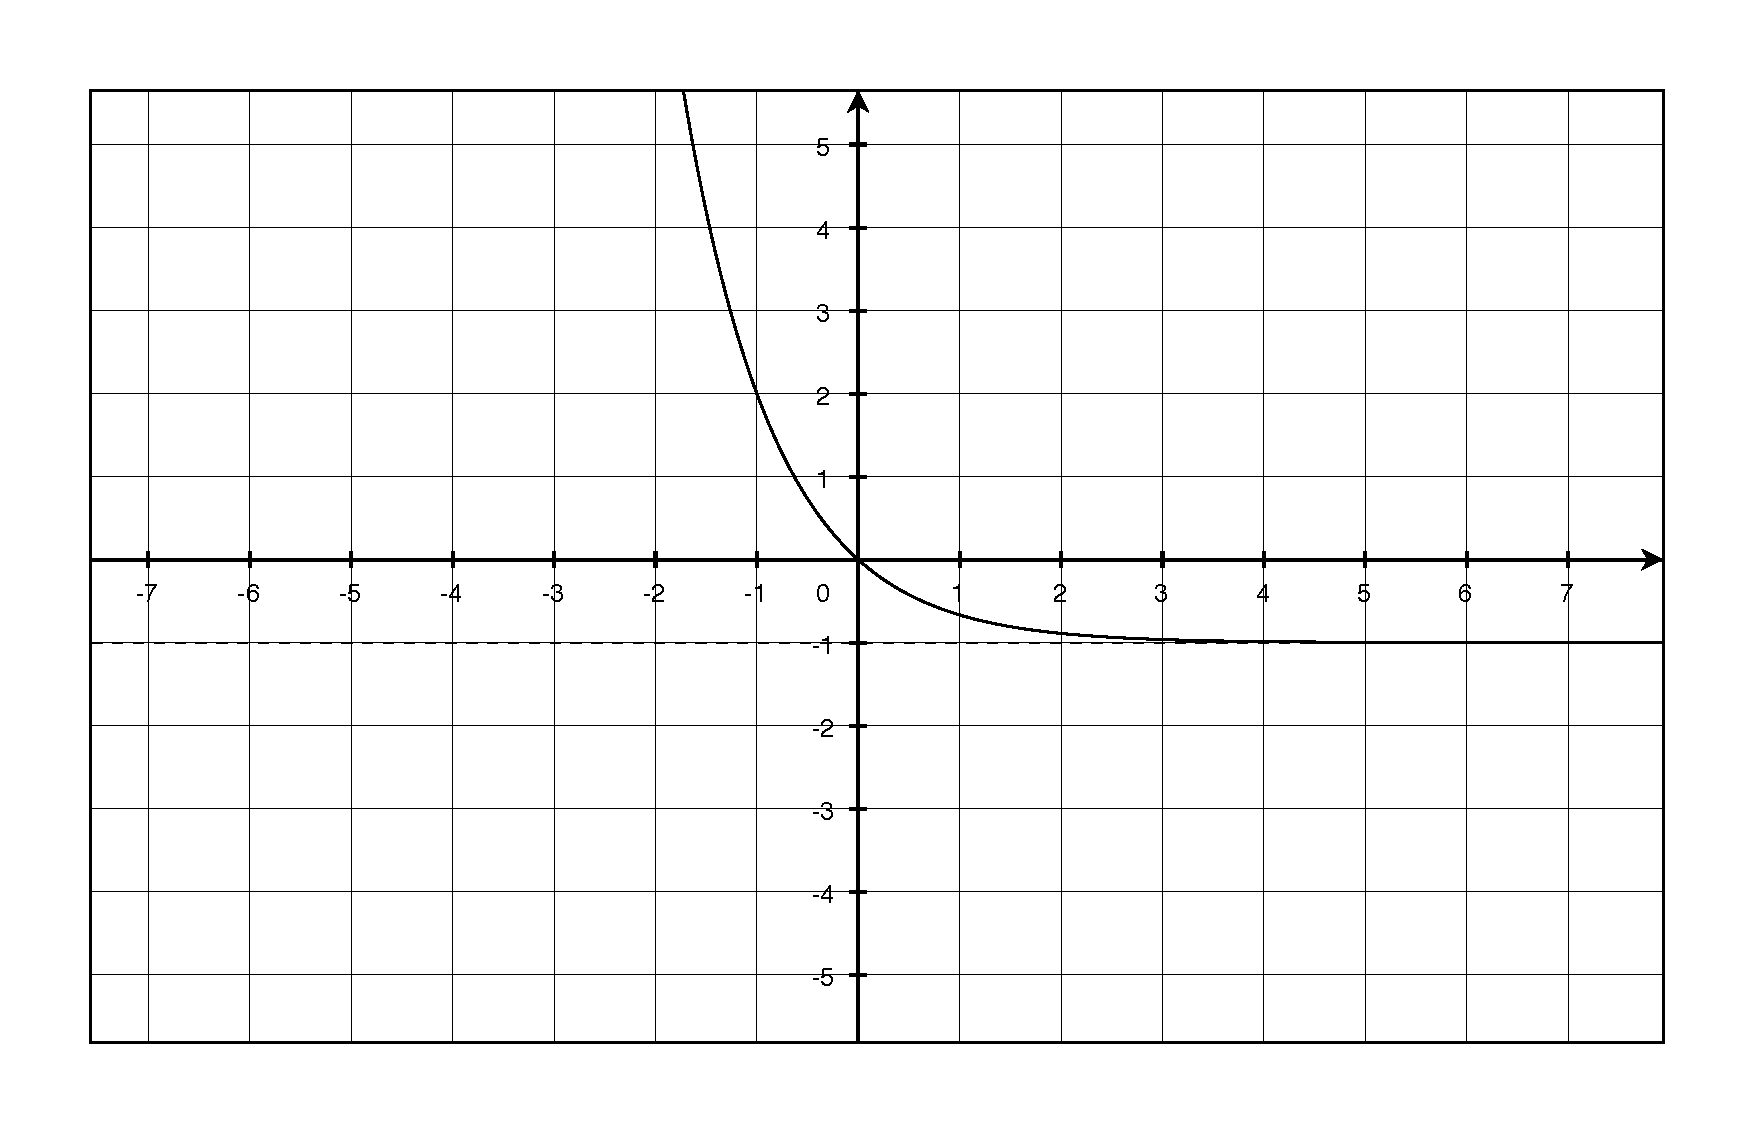
\includegraphics[scale=.5]{final_6.eps}
  \caption*{Question 6}
\end{figure}

\item[Sample Final 7]

I think this problem contains a typo, since Q is mentioned in the instructions but doesn't appear in the equation.

\begin{align*}
  \ln \left[ \frac{3 P^3 R^-2}{P^{1/3}} \right] &= \ln [ 3P^3 R^{-2} P^{-1/3} ] \\
  &= \ln [ 3P^{8/3} R^{-2} ] \\
  &= \ln 3 + \ln P^{8/3} + \ln R^{-2}  \\
  &= \ln 3 + \frac{8}{3} \ln P - 2 \ln R  \\
  &= \ln 3 + \frac{8}{3} a - 2 c  \\
\end{align*}

\item[Sample Final 8]
\begin{description}
\item[a]
In this one, you have to notice that $e^{2x}$ appears in every term and can be factored out.  Since there is no way to
make $e^{2x}$ equal zero, it doesn't affect the solution at all and you just have to solve the quadratic equation that
remains.

\begin{align*}
  x^2e^{2x} - 4xe^{2x} - 5e^{2x} &= 0 \\
  e^{2x} ( x^2 - 4x - 5) &= 0 \\
  e^{2x} (x-5)(x+1) &= 0 \\
\end{align*}

$x = \{-1, 5 \}$

check:
\begin{align*}
  (-1)^2 - 4(-1) - 5 = 1 + 4 - 5 = 0 \\
  5^2 - 4 \cdot 5 - 5 = 25 - 20 - 5 = 0 \\
\end{align*}

\item[b]
\begin{align*}
  e^{2x} - e^x - 2 &= 0 \\
  (e^x - 2)(e^x + 1) &= 0 \\
  \\
  e^x = 2 & \text{ or } e^x = -1 \\
\end{align*}

$e^x = -1$ doesn't provide a solution, so the only solution is $x = \ln 2$

check:
\[
  e^{2 \ln 2} - e^{\ln 2} - 2 = 2^2 - 2 - 2 = 4 - 2 - 2 = 0
\]

\end{description}

\item[Sample Final 14]
You have to memorize the two interest formulas for these.

\begin{description}

\item[a]
\[
  A = 5,000 \left(1 + \frac{0.08}{12} \right)^{12}
\]

\item[b]
\[
  A = 5,000 e^{0.08}
\]

\end{description}

\end{description}


\section{Trigonometry}
\subsection{Things You Should Know}
\begin{itemize}
\item The values of sine, cosine, and tangent for $0$, $\dfrac{\pi}{6}$, $\dfrac{\pi}{3}$, $\dfrac{\pi}{2}$, and $\pi$.
\item The sign of the trigonometric functions in each quadrant.
\item Some identities and laws:
\begin{itemize*}
  \item $\sin^2 x + \cos^2 x = 1$ 
  \item sum of angles formulas
  \item Law of Sines
  \item Law of Cosines
  \item Heron's Formula
  \item $\sin \left( \dfrac{\pi}{2} - 2 \right) = \cos x$, etc.
  \item $\sin (-x) = -\sin x$, etc.
  \item Range of arcsine, arccosine, and arctan
  \item How to solve equations containing trigonometric functions
\end{itemize*}
\end{itemize}

You can derive all the identities if you have a few fundamental identities memorized.  This is probably easier
and less error-prone than trying to memorize all the identities.

For example:
\begin{align*}
  \sin^2 x + \cos^2 x &= 1 \\
  \frac{\sin^2 x}{\sin^2 x} + \frac{\cos^2 x}{\sin^2 x} &= \frac{1}{\sin^2 x} \\
  1 + \cot^2 &= \csc^2 x \\
\end{align*}

or:
\begin{align*}
  \cos(u+v) &= \cos u \cos v - \sin u \sin v \\
  \cos(u+u) &= \cos u \cos u - \sin u \sin u \\
  \cos(2u) &= \cos^2 u - \sin^2 u \\
\end{align*}

If you pick a few to memorize and practice getting some of the others from the ones you plan to have memorized, you
should be in good shape.

\begin{description}

\item[Sample Final 9]

In these, you have to have a few common sines and cosines memorized and then figure out the correct sign.  I drew a
quick picture of each one to figure out the correct quadrant.

\begin{description*}
\item[a] $\sin 120\degree = \dfrac{\sqrt{3}}{2}$
\item[b] $\cos 150\degree = - \dfrac{\sqrt{3}}{2}$
\item[c] $\sin \dfrac{5 \pi}{6} = \dfrac{1}{2}$
\item[d] $\cos\left(- \dfrac{\pi}{6} \right) = \dfrac{\sqrt{3}}{2}$
\end{description*}

\item[Sample Final 10]

\begin{description*}
\item[a] $\cot^{-1}(-\sqrt{3}) = \tan^{-1}(-\dfrac{\sqrt{3}}{3}) = - \dfrac{\pi}{6}$
\item[b] $\sin^{-1} \dfrac{\sqrt{2}}{2} = - \dfrac{\pi}{4}$
\item[c] $\tan^{-1} (-1) = -\dfrac{\pi}{4}$
\item[d] $\cot^{-1} (0) = \dfrac{\pi}{2}$
\end{description*}

\item[Sample Final 11]
You can use the quadratic formula to find the missing side is $2 \sqrt{6}$.  So $\sin x = \dfrac{2\sqrt{6}}{5}$

\item[Sample Final 12]

The first thing to do is to make the problem use all cosines.  We know that 
\[
\sin\left( \dfrac{\pi}{2} - x \right) = \cos x
\]

This problem, however, uses $\sin\left(x - \dfrac{\pi}{2} \right)$.  If you don't remember, what this is, you
can figure out like this:
\begin{align*}
  \sin\left(x - \dfrac{\pi}{2} \right) &= \sin\left[ -\left(\dfrac{\pi}{2} - x \right) \right] \\
  &= - \sin\left(\dfrac{\pi}{2} - x \right) \\
  &= - \cos x
\end{align*}

No we're ready to solve the problem.

\begin{align*}
  2 \cos^2 x - 3 \sin \left(x - \frac{\pi}{2} \right) - 2 &= 0 \\
  2 \cos^2 x + 3 \cos x - 2 &= 0 \\
  (2\cos x - 1)(\cos x + 2) &= 0 \\
  \\
  2 \cos x - 1 = 0     & \text{ or } \cos x + 2 = 0 \\
  \cos x = \frac{1}{2} & \text{ or } \cos x = -2 \\
\end{align*}

$\cos x = \dfrac{1}{2}$ provides the only two solutions.  $\cos x = \dfrac{1}{2}$ when 
\[
  x = \left\{ \frac{\pi}{3} + 2 n \pi, \frac{2 \pi}{3} + 2 n \pi \right\}
\]

\item[Sample Final 13]
For this one, you have to remember Heron's formula.  I had to look it up, so make sure you have it memorized for the
exam.

\[
  A = \sqrt{ \frac{33}{2} \left(\frac{33}{2} - 10 \right) \left(\frac{33}{2} - 15 \right) \left(\frac{33}{2} - 8 \right)}
  = \frac{3}{4}\sqrt{2431}
\]

Simplifying is easiest if you don't multiply everything out.  Factor the numerators and then pull out factors which
appear in pairs.

\end{description}
\section{Conic Sections}

\subsection{Things You Should Know}
\begin{itemize*}
  \item the standard forms of parabola ellipse, hyperbola, circle
  \item how to use {\em complete the square} to put an equation in standard form
  \item the rules for identifying which conic section an equation represents (see below)
\end{itemize*}

The rules for identifying conic sections are very simple.  If $A$ is the coefficient for the $x^2$ term and $B$ is the
coefficient for the $y^2$ term:

\begin{itemize*}
\item if either $A$ or $B$ is zero, you have a parabola
\item if $A$ and $B$ are the same, you have a circle
\item if $A$ and $B$ are different but have the same sign, you have an ellipse
\item if $A$ and $B$ have different signs, you have a hyperbola
\end{itemize*}

Or, another way to say the same thing is:
\begin{itemize*}
\item if $AB = 0$, you have a parabola
\item if $A = B$, you have a circle
\item if $AB > 0$, you have an ellipse
\item if $AB < 0$, you have a hyperbola
\end{itemize*}

\subsection{Sample Problems}

\begin{description}

\item[Sample Final 15]

You can use the rules listed above to classify the equations:

\begin{description*}
\item[a] ellipse
\item[b] hyperbola
\item[c] parabola
\end{description*}

\end{description}

\end{document}

